\documentclass[aps,prmaterials,reprint,onecolumn,amsmath,amssymb,superscriptaddress]{revtex4-2}
\usepackage{siunitx}
\sisetup{range-phrase = --, range-units = single}
\DeclareSIUnit{\rydberg}{Ry}
\DeclareSIUnit{\atomicunits}{a.u.}
%\usepackage{overpic}
\usepackage{graphicx}% Include figure files
\usepackage{graphicx}
\usepackage[abs]{overpic}
%\usepackage{caption}
\usepackage{tikz} 
\usetikzlibrary{calc}
\usepackage{amsmath}
\usepackage{dcolumn}% Align table columns on decimal point
\usepackage{bm}% bold math
%\usepackage[mathlines]{lineno}% Enable numbering of text and display math
%\linenumbers\relax % Commence numbering lines
%\usepackage[a4paper]{geometry}
\usepackage[colorlinks, linkcolor=blue, citecolor=blue, urlcolor=blue]{hyperref}
\usepackage[utf8]{inputenc}
\usepackage[T1]{fontenc}
\usepackage{mathptmx}
\usepackage{etoolbox}
\usepackage{comment}
\usepackage{subcaption}
%\usepackage{nicematrix}
\usepackage{booktabs}
\usepackage{float}
\usepackage{changepage}
\usepackage{xcolor}
\usepackage{float}
\usepackage{bm}
\usepackage{booktabs}
\usepackage{pgfplotstable}
\pgfplotsset{compat=1.18}
\begin{document}

\preprint{AIP/123-QED}

\title[III--V alloy electron mobility]{Calculating electron mobility for III--V alloys In(As$_{1-x}$Sb$_x$), Ga(As$_{1-x}$Sb$_x$) and (In$_{1-x}$Ga$_x$)(As$_{1-x}$Sb$_x$).}% Force line breaks with \\
% Force line breaks with \\
\author{Angus Gentles}
\email{angus.gentles@ams-osram.com}
\affiliation{ams-OSRAM AG, Tobelbader Str. 30, 8141 Premst{\"a}tten, Austria}
\affiliation{Institute for Microelectronics, TU Wien, Gusshausstrasse 27-29, 1040 Wien, Austria}

\author{Mohammad Dehghani}
\thanks{\href{https://orcid.org/0000-0003-4756-0446}{ORCID: 0000-0003-4756-0446}}
\affiliation{Institute for Microelectronics, TU Wien, Gusshausstrasse 27-29, 1040 Wien, Austria}
\affiliation{Christian Doppler Laboratory for Single-Defect Spectroscopy at the
    Institute for Microelectronics, TU Wien, Vienna, Austria}

\author{Dominic Waldh{\"o}r}
\affiliation{Institute for Microelectronics, TU Wien, Gusshausstrasse 27-29, 1040 Wien, Austria}

\author{Pedram Khakbaz}
\affiliation{Institute for Microelectronics, TU Wien, Gusshausstrasse 27-29, 1040 Wien, Austria}
\affiliation{Christian Doppler Laboratory for Single-Defect Spectroscopy at the
    Institute for Microelectronics, TU Wien, Vienna, Austria}
\author{Rainer Minixhofer}
\affiliation{ams-OSRAM AG, Tobelbader Str. 30, 8141 Premst{\"a}tten, Austria}

\author{Michael Waltl}
\affiliation{Institute for Microelectronics, TU Wien, Gusshausstrasse 27-29, 1040 Wien, Austria}

\date{\today}% It is always \today, today,
             %  but any date may be explicitly specified


\maketitle

\begin{figure}
    \centering
    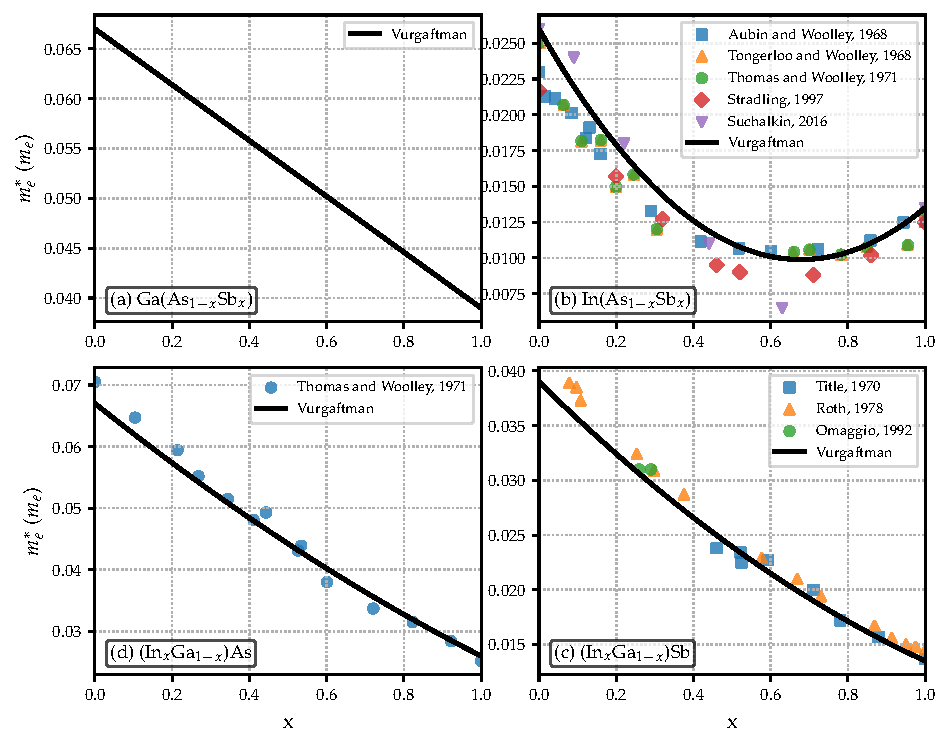
\includegraphics[width=0.8\textwidth]{Figures/meff_exp.pdf}
    \caption{The calculated electron mobility for In(As$_{1-x}$Sb$_x$) (a), Ga(As$_{1-x}$Sb$_x$) (b) and (In$_{1-x}$Ga$_x$)(As$_{1-x}$Sb$_x$) (c) at 300 K, with the alloy scattering contribution shown as a dashed line.}
\end{figure}

\begin{table}[htbp]
\centering
\caption{Fitted parameters and material properties. All experimental results are taken from the Ioffe institute. The $F$'s are the factors associated with the Fr{\"o}hlich interaction in }
\label{tab:results}
\small
\setlength{\tabcolsep}{4pt}
\pgfplotstabletypeset[
  col sep=comma,
  /pgf/number format/fixed,
  /pgf/number format/precision=2,
  /pgf/number format/fixed zerofill,
  empty cells with={--},
  every head row/.style={before row=\toprule, after row=\midrule},
  every last row/.style={after row=\bottomrule},
  columns/name/.style={string type, column name=Material, column type=l},
  columns/x/.style={column name=$x$, /pgf/number format/precision=4, /pgf/number format/fixed zerofill=false},
  columns/y/.style={column name=$y$, /pgf/number format/precision=4, /pgf/number format/fixed zerofill=false},
  columns/UA/.style={column name=$U_A$},
  columns/UB/.style={column name=$U_B$},
  columns/meff_DFT/.style={/pgf/number format/precision=3, column name=$m^*_\mathrm{DFT}$},
  columns/meff_exp/.style={/pgf/number format/precision=3, column name=$m^*_\mathrm{exp}$},
  columns/dielectric_DFT/.style={column name=$\varepsilon_{\infty,\mathrm{DFT}}$},
  columns/dielectric_exp/.style={column name=$\varepsilon_{\infty,\mathrm{exp}}$},
  columns/omega_TO_DFT/.style={column name=$\omega_{\mathrm{TO,DFT}}$},
  columns/omega_TO_exp/.style={column name=$\omega_{\mathrm{TO,exp}}$},
  columns/omega_LO_DFT/.style={column name=$\omega_{\mathrm{LO,DFT}}$},
  columns/omega_LO_exp/.style={column name=$\omega_{\mathrm{LO,exp}}$},
  columns/F_DFT/.style={column name=$F^\text{Fr}_\mathrm{DFT}$},
  columns/F_exp/.style={column name=$F^\text{Fr}_\mathrm{exp}$},
  columns/F_ratio/.style={column name=$F^\text{Fr}_\mathrm{DFT}/F^\text{Fr}_\mathrm{exp}$},
]{data/results_summary.csv}
\end{table}

\end{document}
